\chapter{Sistemas de Información Geográfica}
Con el transcurrir del tiempo se ha tratado de representar la superficie terrestre y los elementos
que esta alberga. Los primeros mapas, que no presentaban un alto grado de exactitud, eran
utilizados como herramienta para la navegación. Con el paso del tiempo los requerimientos fueron
creciendo, surgiendo así la necesidad de mejorar la precisión en las mediciones y la inclusión de
elementos adicionales con el fin de modelar, recursos, fenómenos naturales y asentamientos humanos
en la superficie.

Los sistemas de información geográfica o SIG, surgen ante la necesidad de registrar, procesar y
analizar la información geográfica de forma más eficiente. Se encuentra principalmente compuesto
por la información geográfica y herramientas correspondientes para su gestión y análisis. En este
capítulo se introduce a los sistemas de información geográfica, la representación de datos
geoespaciales y los métodos de interpolación como herramienta para análisis espacial.

%##Capítulo 2. Sistemas de Información Geográfica
%* Introducción
%* Estructuras de datos de los Sistemas de Información Geográfica
\section{Definición de Sistema de información geográfica}
\label{sec:cap2-definicion-sig}

Un Sistema de Información geográfica o SIG (por sus siglas en español), según \cite{lopezMarcos2007} es 
\textit{"la integración organizada de hardware, software y datos geográficos diseñada para almacenar, manejar,
capturar, analizar y desplegar la información geográficamente de múltiples formas, con el fin de resolver problemas
de planificación y gestión geográfica. También puede definirse como un modelo de una parte de la realidad referido
a un sistema de coordenadas terrestre y construido para satisfacerunas necesidades concretas de información"}.

Se basan en los principios formales de matemáticas discretas, modelos de datos y geometría computacional; su
desarrollo, en nuevas tecnologías de la información: estándares e ingeniería de software, almacenes de datos, 
Web-SIG, metadatos, ambientes y lenguajes visuales, graficación entre muchas otras\cite{lunaPaulina2010}.

La característica principal de los SIG es el manejo de datos complejos basados en datos geométricos (coordenadas e
información topológica) y datos de atributos (información nominal) la cual describe las propiedades de los objetos
geométricos tales como punto, lineas y polígonos. En la actualidad las funciones básicas, y más habitualmente
utilizadas, de un SIG son el almacenamiento, visualización, consulta y análisis de datos espaciales. Un uso
más avanzado sería la utilización de un SIG para la toma de decisiones en ordenación territorial o para la
modelización de procesos ambientales.

\begin{itemize}
    \item  Almacenamiento : el almacenamiento de datos espaciales implica modelizar la realidad y codificar de
    forma cuantitativa este modelo.

    \item Visualización : La información se presenta en un espacio de cuatro dimensiones (3 espaciales y el tiempo) 
    pero debido al peso que la tradición cartográfica tiene sobres los SIG, una de las formas prioritarias de 
    presentación de los datos es en su proyección sobre el espacio bidimensional definido mediante coordenadas cartesianas.
    
    \item Consultas  : en una base de datos, las consulta se basan en propiedades temáticas,mientras que en un SIG 
    las consultas se basan tanto en atributos temáticos como en propiedades espaciales.

    \item Análisis :  el uso de herramientas de análisis espacial y álgebra de mapas para el desarrollo y
    verificación de hipótesis acerca de la distribución espacial de las variables y objetos.

    \item Toma de decisiones : la utilización de un SIG para resolver problemas de toma de decisión en
    planificación física, ordenación territorial, estudios de impacto ambiental, etc.

    \item Modelización : las aplicaciones más elaboradas de los SIG son aquellas relacionadas con la integración 
    de modelos matemáticos de procesos naturales, dinámicos y espacialmente distribuidos.
\end{itemize}

%* Sistemas de proyección
\section{Sistemas de proyección}
\label{sec:cap2-sistemas-de-proyeccion}

Durante el siglo XVII, cartógrafos especializados como Mercator demostraron que no sólo el uso de un sistema de
proyección matemático y un ajustado sistema de coordenadas mejoraba la fiabilidad de las medidas y la localización
de las áreas de tierra, sino que el registro de fenómenos espaciales a través de un modelo convenido de
distribución de fenómenos naturales y asentamientos humanos era de un valor incalculable para la navegación, para
la búsqueda de rutas y en la estrategia militar \cite{llopis2006sistemas}.

\subsection{Coordenadas geográficas}
Las coordenadas geográficas proveen un sistema de referencia que utilizan coordenadas angulares (latitud y
longitud) cuyo fin es el de determinar los ángulos laterales de la superficie terrestre. La latitud es el ángulo
que existe entre un punto cualquiera y el Ecuador, medida sobre el meridiano que pasa por dicho punto. La longitud
mide el ángulo a lo largo del ecuador desde cualquier punto de la Tierra.

Para la representación de objetos puntuales en una superficie, se utilizan las coordenadas X e Y que caracterizan
la planimetría y una coordenada Z que representa la altimertría del objeto en cuestión. 

\subsection{Proyecciones}
Se denomina proyecciones cartográficas o proyecciones geográficas al conjunto de métodos utilizados para establecer
una correspondencia matemática entre los puntos de la superficie curva de la tierra y sus transformaciones en una
superficie plana. 

El problema principal a la hora de realizar una proyección es que no existe forma de representar un una superficie
plana toda la superficie curva, de la tierra, sin deformarla. Teniendo en cuenta que la curvatura de la superficie
terrestre es proporcional al tamaño del área representada, esta deformación solo es relevante para zonas muy
amplias. Si el área representada es pequeña, como ciudad, la deformación o distorsión es despreciable por lo que
comúnmente son utilizadas coordenadas planas, relativas a un origen de coordenadas arbitrario y medidas sobre el
terreno.

Con la aparición y difusión de los SIG, el conjunto de herramientas que ofrece dio paso a posibilidad de combinar
información de diferentes mapas con diferentes proyecciones, esto ha incrementado la relevancia de la cartografía 
más allá de la simple confección de mapas.

\subsection{Elementos de representación cartográfica}
Para representar un objeto cualquiera o un fenómeno geográfico en un mapa es fundamental conocer las
características de este dato que contempla los tres aspectos siguientes: dimensiones, nivel de medida y
distribución. El análisis de las características de los elementos permite elegir la simbología más adecuada para
representar los fenómenos geográficos.
 
A cada entidad espacial se puede asociar diversas variables han desarrollado un amplio conjunto de técnicas para
cartografiar los hechos de la superficie terrestre.

\subsubsection{Dimensiones}
Por su extensión, los fenómenos que se representan en un mapa pueden clasificarse como puntuales, lineales,
poligonales o espacio-temporales.

\begin{itemize}
    \item Fenómenos puntuales : indican la presencia de entidades de un modo puntual. Pueden representarse
    utilizando diferentes símbolos o colores para una variable cualitativa, o diferentes tamaños para variables
    cuantitativas.
    
    \item Fenómenos lineales : simbolizan entidades, naturales o artificiales, de forma lineal conformadas a
    partir de la unión de varios puntos. Pueden utilizarse diferentes anchuras de linea, diferentes colores o
    diferentes tipos de linea para representar propiedades como la anchura de los ríos o categorías de vías de
    comunicación.
        
    \item Fenómenos Poligonales : La información puede ser bidimensional o tridimensional, que, por su tamaño,
    pueden ser representados como polígonos o porciones homogéneas del terreno en relación a una variable
    cualitativa. Pueden utilizarse diferentes colores o tramas para representar variables cualitativas o
    cuantitativas.

    \item Fenómenos espacio-temporales : La información depende del movimiento del fenómeno con respecto al paso
    del tiempo (migraciones de aves, expansión de una civilización,etc.).
\end{itemize}

\subsubsection{Nivel de medida}
Los elementos de la naturaleza se miden con el fin de clasificarlos y compararlos; lo que no siempre implica una
magnitud cuantitativa, ya que puede ser cualitativa u jerárquica. En orden creciente de precisión tenemos:
\begin{itemize}
    \item Escala nominal : asigna una característica no numérica a un fenómeno, por lo que sólo se pueden hacer 
    comparaciones de tipo cualitativo. Por ejemplo, un mapa de cuencas hidrográficas, un mapa de suelos. 
    Este es el nivel más elemental de medida, pues no informa acerca de la cantidad o el orden.
    
    \item Escala ordinal : establece una cierta jerarquía no mensurable o no cuantificable entre los diferentes
    elementos. Por ejemplo, un mapa en el que aparecen núcleos de población, cuyos símbolos están jerarquizados
    según el número de habitantes sin especificar cantidad.
    
    \item Escala cuantitativa o de intervalo : La escala cuantitativa o de intervalo asigna una característica 
    numérica a un fenómeno geográfico. Por ejemplo, en un mapa de temperaturas medias los intervalos son valores 
    numéricos (expresados en grados Celsius o Fahrenheit). Es necesario emplear algún tipo de unidad convencional.
\end{itemize}

\subsubsection{Distribución}
La ocurrencia de un fenómeno sobre una superficie terrestre puede darse a lo largo y ancho de toda ella, o de
forma discontinua, dándose el fenómeno en alguna localización del territorio. Los fenómenos en cuestión son :

\begin{itemize}
    \item Fenómenos continuos :  son los que tienen presencia en todos los puntos del territorio objeto de 
    representación, aunque sólo se tengan medidas de algunos puntos significativos. Por ejemplo: la temperatura,
    altitud sobre en nivel del mar, niveles de contaminación atmosférica,densidad poblacional, etc.
    
    \item Fenómenos discretos : son los que tiene presencia en algunos puntos del territorio objeto de 
    representación. Un ejemplo son los datos de población, dado que se localizan en determinadas áreas y 
    no en todos los puntos del territorio. Algunos fenómenos discretos pueden transformarse en continuos mediante 
    la aplicación de una relación. Por ejemplo, el número de habitantes de una provincia (fenómeno discreto) pasa
    a ser un fenómeno continuo cuando se habla de densidad de población: la relación se aplica dividiendo el
    número de habitantes por la superficie de la provincia en $km^2$
\end{itemize}

%* Técnicas gráficas de representación
\section{Representación de los datos }
\label{sec:cap2-tecnicas-graficas-representacion}
Los objetos del mundo real se pueden describir mediante los fenómenos discretos y continuos, donde las variables y objetos se muestrean y organizan para lograr una representación adecuada. En un
SIG existen básicamente dos modelos lógicos que se conocen como formato ráster y formato vectorial
y que dan lugar a los dos grandes tipos de capas de información espacial \cite{fAlonsoSig2006}.

\subsection{Formato ráster}
El formato ráster se centra en las propiedades del espacio más que en la precisión de la
localización. Divide el espacio en un conjunto regular de celdas, donde cada una contiene un
número que puede ser el identificador de un objeto o del valor de una variable
\cite{fAlonsoSig2006}. Se trata de un modelo de datos muy adecuado para la representación de
variables continuas en el espacio.

Los datos ráster se encuentran definidas como una grilla con un número determinado de filas y
columnas, donde a celda se le asocia un único valor. Los datos ráster pueden ser imágenes, donde
el valor asociado a cada celda o píxel de la imagen, representa un color. Otros valores
registrados para cada celda puede ser un valor discreto o un valor nulo para indicar que no se
disponen datos.

\begin{figure}[!htbp]
\centering
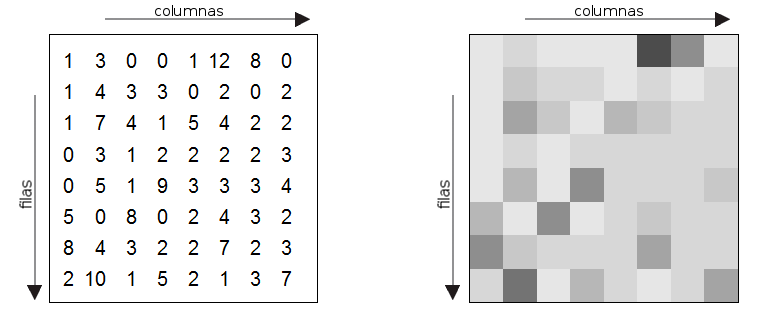
\includegraphics[width=0.9\textwidth]{capitulo-2/graphics/representacion-raster.png}
\caption{\label{fig:sig-capa-raster} Comparación entre la definición de una capa ráster y su representación. }
\end{figure}

La resolución y la nitidez del la capa ráster depende del tamaño de la celda
(\figref{fig:sig-raster-resolucion}), donde el tamaño esta asociado a la cantidad de columnas y
filas de la capa ráster. Mientras más filas y columnas cuente una capa ráster, más nítida será la
imagen resultante.


\begin{figure}[!htbp]
    \centering
    \begin{subfigure}[b]{0.4\textwidth}
            
\includegraphics[width=\textwidth]{capitulo-2/graphics/raster-baja-resolucion.png}
            \caption{Tamaño de celda inadecuado, imágen de baja resolución.}
    \end{subfigure}
    ~~~~
    \begin{subfigure}[b]{0.4\textwidth}
            
\includegraphics[width=\textwidth]{capitulo-2/graphics/raster-alta-resolucion.png}
            \caption{Tamaño de celda adecuado, imágen de alta resolución.}

    \end{subfigure}
    \caption{\label{fig:sig-raster-resolucion}Curvas de nivel rasterizadas con dos tamaños distintos de celdas y su relación con la resolución de las imagenes resultantes (Tomado de \cite{fAlonsoSig2006}).}
\end{figure}

\subsection{Formato vectorial}
Los datos vectoriales, se caracterizan por la precisión de localización de los elementos
geográficos en el espacio, donde los fenómenos a representar son discretos, con límites bien
definidos. Generalmente se considera que el formato vectorial es más adecuado para la
representación de entidades o variables cualitativas y el formato ráster para representar
superficies\cite{fAlonsoSig2006}.

Los diferentes objetos, vectoriales, se encuentran representados como puntos, lineas o polígonos
\cite{fAlonsoSig2006}. De tal forma que para modelar digitalmente las entidades del mundo real se
utilizan estos tres elementos geométricos.

\begin{figure}[!htbp]
\centering
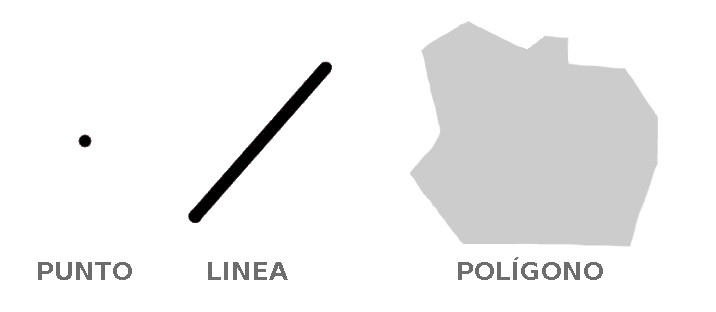
\includegraphics[width=0.8\textwidth]{capitulo-2/graphics/dimensiones-datos.jpg}
\caption{\label{fig:sig-xyz} Elementos geométricos utilizados para modelar digitalmente las entidades en un SIG.}
\end{figure}

\begin{itemize}
    \item \textit{Puntos} : se utilizan para representar las entidades geográficas que pueden ser
    descritas como un fenómeno puntual. Estos transmiten la menor cantidad de información y su representación es la más simple.

    \item \textit{Líneas o polilíneas} : las líneas unidimensionales o polilíneas son usadas para
    representar elementos con rasgos lineales como ríos, caminos, ferrocarriles, rastros, líneas
    topográficas o curvas de nivel.

    \item \textit{Polígonos} : se utilizan para representar elementos geográficos que cubren un
    área particular de la superficie de la tierra. Los polígonos transmiten mayor cantidad de
    información y en ellos se pueden medir el perímetro y el área.
\end{itemize}

\subsection{Ventajas y desventajas de los formatos ráster y vectorial}

El debate acerca de la conveniencia de uno u otro modelo debe basarse en el tipo de estudio o
enfoque que se quiera hacer, pero también del software y fuentes de datos disponibles
\cite{fAlonsoSig2006}.

El formato ráster se considera el más adecuado para representar eficientemente las superficies.
Estas solo pueden representarse vectorialmente mediante modelos híbridos que no resultan adecuados
para la realización de posteriores análisis ya que todas las operaciones que permite el modelo
ráster resultan más lentas con el modelo vectorial \cite{fAlonsoSig2006}. Tradicionalmente se ha
considerado que para la representación de los objetos resulta más eficiente la utilización de un
formato vectorial ya que la estructura de los datos es compacta y almacena los datos sólo de los
elementos digitalizados por lo que requiere menos memoria para su almacenamiento y tratamiento
\cite{fAlonsoSig2006}. Los gráficos vectoriales, se caracterizan por no perder la definición a
media que se aumenta la escala para la visualización.

\begin{figure}[!htbp]
    \centering
    \begin{subfigure}[b]{0.4\textwidth}
            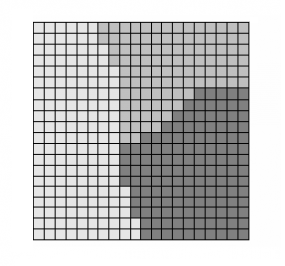
\includegraphics[width=\textwidth]{capitulo-2/graphics/formato-raster.png}
            \caption{Formato ráster.}
    \end{subfigure}
    ~~~~
    \begin{subfigure}[b]{0.4\textwidth}
            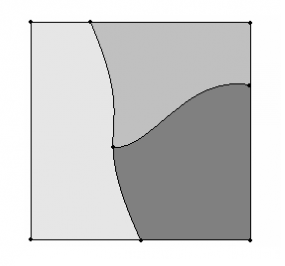
\includegraphics[width=\textwidth]{capitulo-2/graphics/formato-vectorial.png}
            \caption{Formato vectorial.}

    \end{subfigure}
    \caption{\label{fig:sig-raster-vs-vectorial} Representación de una misma superficie, mediante los formatos ráster y vectorial, en un SIG.}
\end{figure}

En general las ventajas del modelo ráster radican en, su simplicidad y la velocidad de ejecución de
los operadores lo que lo convierte en el modelo a utilizar para la representación de modelos
digitales de terreno o imágenes satelitales. Por otro lado, entre sus desventajas podemos
mencionar su inexactitud que depende de la resolución y el tamaño de las celdas, además podemos
mencionar que se requiere una gran cantidad de espacio para el almacenamiento aunque este problema
puede compensarse mediante diversos sistemas de compresión.

Hoy en día se pueden codificar las formas en un modelo vectorial y los procesos con un modelo
ráster, para ello se requieren herramientas eficaces de paso de un formato al otro. Resulta
sencillo, finalmente, la visualización simultánea de datos en los dos formatos gracias a la
capacidad gráfica actual\cite{fAlonsoSig2006}.

%* Análisis espacial con SIG
\section{Análisis espacial en un SIG}
\label{sec:cap2-analisis-espacial-sig}

Un SIG puede reconocer y analizar las relaciones espaciales que existen en la información geográfica almacenada.
Estas relaciones topológicas permiten realizar modelizaciones y análisis espaciales complejos. Así, por ejemplo, 
el SIG puede discernir la parcela o parcelas catastrales que son atravesadas por una línea de alta tensión, o bien
saber qué agrupación de líneas forman una determinada carretera.

En suma podemos decir que en el ámbito de los sistemas de información geográfica se entiende como topología a las 
relaciones espaciales entre los diferentes elementos gráficos (topología de nodo/punto, topología de red/arco/línea, 
topología de polígono) y su posición en el mapa (proximidad, inclusión, conectividad y vecindad). Estas relaciones, 
que para el ser humano pueden ser obvias a simple vista, el software las debe establecer mediante un lenguaje y unas
reglas de geometría matemática.

Para llevar a cabo análisis en los que es necesario que exista consistencia topológica de los elementos de la base de 
datos suele ser necesario realizar previamente una validación y corrección topológica de la información gráfica. 
Para ello existen herramientas en los SIG que facilitan la rectificación de errores comunes de manera automática o 
semiautomática.

La geoestadística analiza patrones espaciales con el fin de conseguir predicciones a partir de datos espaciales concretos.
Es una forma de ver las propiedades estadísticas de los datos espaciales. A diferencia de las aplicaciones estadísticas 
comunes, en la geoestadística se emplea el uso de la teoría de grafos y de matrices algebraicas para reducir el número de 
parámetros en los datos. Tras ello, el análisis de los datos asociados a entidad geográfica se llevaría a cabo en segundo 
lugar.

Cuando se miden los fenómenos, los métodos de observación dictan la exactitud de cualquier análisis posterior. Debido a 
la naturaleza de los datos (por ejemplo, los patrones de tráfico en un entorno urbano, las pautas meteorológicas en el 
océano, etc.), grado de precisión constante o dinámico se pierde siempre en la medición. Esta pérdida de precisión se 
determina a partir de la escala y la distribución de los datos recogidos. Los SIG disponen de herramientas que ayudan a 
realizar estos análisis, destacando la generación de modelos de interpolación espacial.


%* Métodos de interpolación
\section{Métodos de interpolación}
\label{sec:cap2-metodos-interpolacion}

La interpolación espacial, consiste en la utilización de puntos con valores conocidos, también denominados puntos
de control, para estimar una variable en lugares donde se desconoce; también se considera una forma de transformar
información puntual en información de superficie, con el objetivo de combinarla con otros datos para facilitar el
análisis y la modelado espacial.

Todos los métodos de interpolación se basan en la presunción lógica de que cuanto más cercanos están dos puntos
sobre la superficie terrestre, los valores de cualquier variable cuantitativa que midamos en ellos serán más
parecidos, para expresarlo más técnicamente, las variables espaciales muestran autocorrelación espacial \cite{fAlonsoSig2006}.

El resultado de la interpolación espacial depende de un algoritmo computacional o una ecuación matemática en la
cual se emplean los datos de los puntos de control\cite{NINO2011}.


\subsection {Red de Triángulos Irregulares (TIN)}
Las Redes Irregulares de Triángulos (TIN por sus siglas en ingles Triangulated Irregular Network), se generan a
partir de valores puntuales tratando de conseguir triángulos que maximicen la relación área/perímetro, el conjunto
de todos los triángulos forma un objeto geométrico denominado conjunto convexo\cite{fAlonsoSig2006}. Son
ampliamente utilizados como método para la representación de modelos de elevaciones, ya que producen resultados
visualmente muy buenos, sin embargo a la hora de realizar la integración con la información raster restante, se
necesita interpolar una capa raster a partir de los triángulos.

Según \cite{cPachecoMDE2003} TIN utiliza los puntos de entrada para construir una red de triángulos según el
criterio de Delauny: en cada triángulo, el círculo que pasa a través de los tres vértices no encierra ningún otro
punto de entrada (el criterio de Delauny genera, tanto como le es posible, triángulos pequeños y equiláteros y es
ley ser utilizado para crear objetos TIN). Luego, el proceso ajusta una superficie plana a cada triángulo, de
manera tal que el total de la superficie está modelada como una colección de facetas trianguladas planas.


\begin{figure}
\centering
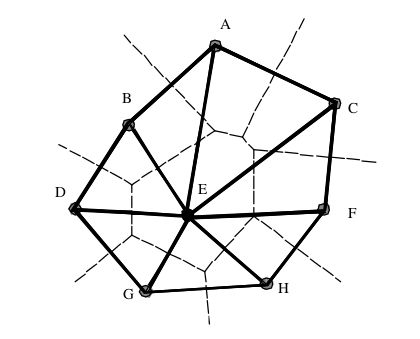
\includegraphics[width=0.4\textwidth]{capitulo-2/graphics/TIN-cPachecoMDE2003.png}
\caption{\label{fig:sig-tin}Red de Triángulos Irregulares (TIN) (Tomado de \cite{cPachecoMDE2003}).}
\end{figure}


\subsection{Ponderación de la inversa de la distancia (IDW)}
Estima los puntos del modelo realizando una asignación de pesos a los datos del entorno en función inversa a la
distancia que los separa del punto en cuestión. De esta forma, se acepta que los puntos más próximos al centroide
intervienen de manera más relevante en la obtención del valor definitivo de Z para ese punto.

La elección del exponente de ponderación(p) determina la contribución de los puntos circundantes al punto 
problema, cuanto mayor es p, más contribuyen los puntos próximos. Es necesario contar con muchos puntos para la
interpolación.

La forma general de encontrar un valor interpolado $u$ en un punto $x$ basado en muestras $u_i = u (x_i)$ para 
$i = 0,1, ..., N$ utilizando IDW es una función de interpolación:

\begin{equation}\label{eq:interpolacion-idw}
 u(x) = \sum_{i=1}^{N} \frac{w_i(X)}{\sum_{j=1}^{N} w_j(X)}
\end{equation}

donde 

\begin{equation} 
w_i(X) =  \frac{1}{d(X, X_i)^p} 
\end{equation}

\subsection{Kriging}
El Kriging es un método geoestadístico de interpolación espacial de carácter global, exacto y estocástico. La 
idea básica de este método corresponde a la noción de dependencia espacial, según la cual las muestras cercanas
tienen mayor similitud entre sí que las más apartadas\cite{NINO2011}.

Se presenta con un método de interpolación con una expresión general similar a la anterior (IDW). La diferencia
básica es que asume que la altitud puede definirse como una variable regionalizada. Supone que la variación
espacial de la variable a representar puede ser explicada al menos parcialmente mediante funciones de correlación
espacial(la variación espacial de los valores de z puede deducirse de los valores circundantes de acuerdo con unas
funciones homogéneas en toda el área).

%* Aplicaciones de SIG y análisis epidemiológicos
\section{Aplicaciones y análisis epidemiologico}
\label{sec:cap2-aplicaciones-analisis-epidemiologico}

Con el correr del tiempo su el potencial ha incrementado rápidamente, desde su concepción en los años setenta,
actualmente las áreas en las que se aplica se ha diversificado, entre las más resaltantes podemos nombrar:
biología, energía e infraestructura, planificación urbana y regional, monitoreo ambiental y geografía física,
transportación y logística. Entre las aplicaciones más usuales destacan las del campo científico, gestión 
y empresarial. 

Las autoridades sanitarias, en sus tareas de vigilancia en Salud Pública, tienen en los GIS una 
herramienta fundamental para conocer cómo se extiende una enfermedad, estudiar su posible relación 
con un potencial foco de riesgo, o localizar un brote epidémico\cite{vgomesAegis2001}. 

Los análisis más utilizados por las entidades sanitarias son la cartografía de enfermedades, cuyo fin es
representar la distribución espacial de la enfermedad,  y el análisis de focos de riesgo, que establece 
bandas alrededor de un punto o una zona geográfica representando una potencial fuente contaminante para 
comparar el riesgo de una enfermedad en cada una de esas bandas. La información necesaria para realizar 
este tipo de estudios proviene de muy diversas fuentes: registros de mortalidad, hospitales, facultativos, 
bases de datos oficiales, observatorios medioambientales o meteorológicos, proyectos específicos. Por 
tanto, es muy importante recopilar y tratar de forma unificada toda esta información para facilitar su 
acceso y análisis.

Los SIG son capaces de simplificar grandes tareas como la localización de eventos en espacio y tiempo, 
el monitoreo de eventos de salud y el comportamiento de factores de riesgo en un período de tiempo dado, la
identificación de áreas geográficas y grupos de población con grandes necesidades de salud y contribuye a la
solución de tales necesidades mediante el análisis de múltiples variables y la evaluación del impacto de
intervenciones en salud\cite{iMolinaSigEpidemiologia}.

\section{Vigilancia entomológica del dengue}
\label{sec:gis-vigilancia-entomologica-dengue}
La vigilancia entomológica del vector, el Aedes aegypti, se utiliza con propósitos operativos, y de
investigación, para determinar los cambios en la distribución geográfica del vector, la vigilancia
y evaluación de los programas de control, obtener medidas relativas de la población del vector en
el tiempo, y facilitar la toma de decisiones \cite{world2009dengue}, con el fin de disminuir
población del vector \cite{world2009dengue,dengueUruguayCap1, cenaprece2013,NINO2011}.

El análisis de la distribución espacial y temporal de las poblaciones del vector, puede llegar a
jugar un papel importante en la planificación y evaluación de medidas orientadas a la disminución
de las poblaciones del vector y en consecuencia, reducir los casos de dengue
\cite{world2009dengue,dengueUruguayCap1, cenaprece2013,nino2008uso}. Los SIG constituyen una
herramienta esencial para el análisis de la distribución espacial de las poblaciones
\cite{vgomesAegis2001,petric2012surveillance}, permitiendo obtener mejores resultados en
combinación con las metodologías de vigilancia entomológica y médicas\cite{petric2012surveillance}.

La utilización de los GIS permite hacer un análisis rápido para determinar anticipadamente las
intervenciones mas adecuadas que eviten o disminuyan el desarrollo de
epidemias\cite{bottinelli2002estratificacion}. Si bien el estudio es preliminar, permite
apreciar perfectamente las áreas de mayor riesgo de transmisión del virus del dengue\cite{bottinelli2002estratificacion, NINO2011}.

Los métodos de muestreo, como larvitrampas y ovitrampas resultan eficientes y económicos para
determinar determinar la distribución espacial y temporal del Aedes aegypti y otros mosquitos
\cite{dengueUruguayCap1, cenaprece2013}.


%!TEX root = ../tesis.tex
\subsection{Identificación de focos de infestación del dengue}
\label{sec:cap4-identificacion-focos}
Las metodologías de vigilancia entomológica basadas en la distribución geográfica de larvitrampas
u ovitrampas, como las presentadas en
\cite{NINO2011,petric2012surveillance, journal.pone.0054167,nino2008uso}, permiten generar
información regionalizada sobre la abundancia poblacional del vector. Los datos
sobre los mosquitos recolectados deben mantenerse para crear un registro histórico de las
especies de mosquitos que se encuentran en asociación con diferentes hábitats y patógenos para
permitir la detección temprana de las adaptaciones \cite{petric2012surveillance}.

En \cite{NINO2011} se propone una metodología de vigilancia entomológica basada en la utilización
de larvitrampas para la identificación de focos de intestación del dengue, donde las larvitrampas
deben ser distribuidas geográficamente (\figref{fig:sig-distribucion-puntos-control}) para generar
información regionalizada correspondiente al área de estudio. Las técnicas de
interpolación espacial permiten transformar la información regionalizada en mapas de
interpolación (\figref{fig:sig-puntos-control-interpolacion}), donde se puede apreciar los niveles
de infestación del vector del dengue, y el riesgo correspondiente a la abundancia de mosquitos
observada en el área de estudio \cite{NINO2011}. El hecho de contar con esta información
regionalizada permitirá a las autoridades pertinentes definir y planificar mejor las medidas de
prevención y control a realizarse para reducir los niveles de infestación en las zonas criticas
\cite{NINO2011, nino2008uso, petric2012surveillance}.

\begin{figure}[!htbp]
\centering
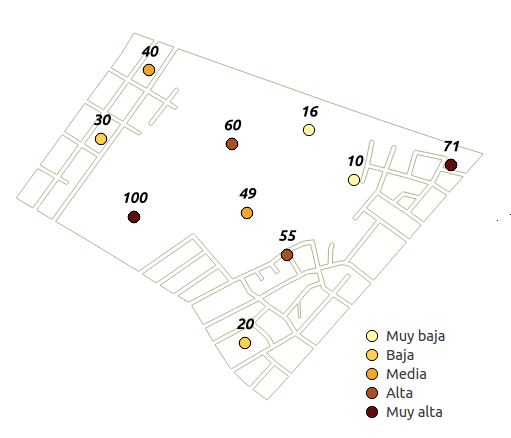
\includegraphics[width=1\textwidth]{capitulo-2/graphics/distribucion-puntos-control.png}
\caption{\label{fig:sig-distribucion-puntos-control}Ejemplo de disposición de larvitrampas (azul) y abundancia de larvas (rojo) (Tomado de \cite{NINO2011}).}
\end{figure}

Los mapas de interpolación resultantes, indican, con mayor detalle que los índices aédicos
tradicionales, los lugares específicos donde sería necesario tomar medidas de prevención y
control de acuerdo al grado de infestación, permitiendo así una mayor racionalización de tiempo y
recursos \cite{NINO2011}.

\begin{figure}[!htbp]
\centering
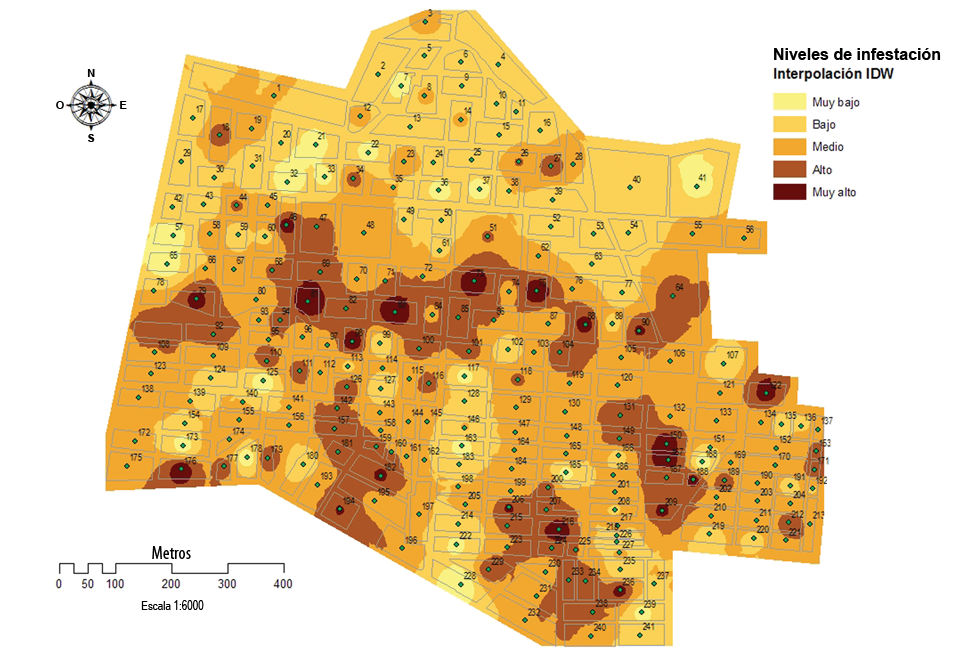
\includegraphics[width=1\textwidth]{capitulo-2/graphics/puntos-control-interpolacion.png}
\caption{\label{fig:sig-puntos-control-interpolacion}Ejemplo de mapa de interpolación resultantes (Tomado de \cite{NINO2011}).}
\end{figure}


